\chapter{Algoritmo Propuesto}
\label{sec:modeloOpti}
%dado que se tienen muchos filamentos, se debe evaluar cual es mejor. Explicar como propiedades topológicas y geométricas tienen. Y como se ponderan para un peso que será minimizado o maximizado

En base a lo recopilado en los cap\'itulos previos de esta investigaci\'on, es posible destacar los siguientes aspectos del problema a resolver:

\begin{itemize}
    \item Se desconoce a priori el n\'umero de filamentos a buscar.%, dado que una imagen puede tener individualizaciones distintas para 2 expertos.
    \item Generalmente se busca individualizar m\'as de un filamento por imagen, lo que conlleva a elegir los mejores filamentos entre las soluciones que se encuentren.
    \item El uso de un grafo para representar la red de filamentos puede implicar que las combinaciones de soluciones crezcan de manera exponencial.
\end{itemize}

Lo anterior permite clasificar el problema de identificar filamentos a partir de un grafo como un problema de optimizaci\'on con restricciones \citepxl{blum2011hybrid}.


%\section{Individualizaci\'on de filamentos mediante la metaheur\'istica ACO}
%similitud entre ambos
Se ha establecido en la secci\'on \ref{sec:OptiMethods} que una red de filamentos puede ser representada mediante un grafo, de forma similar a lo que sucede con la representaci\'on del conjunto de caminos que las hormigas recorren en b\'usqueda de alimento. En particular, un filamento en un grafo corresponde a un conjunto de aristas adyacentes, con lo que se puede asociar la individualizaci\'on de un filamento a la elecci\'on de una o m\'as aristas o componentes de soluci\'on, tal como se lleva a cabo en la metaheur\'istica ACO. A su vez, durante la elecci\'on de las aristas adyacentes que permiten individualizar un filamento, se puede utilizar una o m\'as caracter\'isticas que las aristas o componentes de soluci\'on poseen, para dirimir entre las aristas a elegir durante este proceso. Este comportamiento es similar al que las hormigas realizan utilizando las feromonas. Lo anterior constituye el fundamento para utilizar la metaheur\'istica ACO en el proceso de construcci\'on y evaluaci\'on de soluciones que permiten individualizar filamentos.

%Problema de explorar el espacio de soluciones
%comportamiento de las hormigas se puede asemejar a la forma en que los filamentos fueron creciendo o decreciendo.
La b\'usqueda de conjuntos de aristas adyacentes para individualizar uno o m\'as filamentos implica examinar un espacio de soluciones que no es posible de recorrer en tiempo polinomial, dado que sin restricciones las combinaciones crecen exponencialmente \citepxl[ver\hspace{0.1cm} ]{buchin2007number, biswas2012hamiltonian}. La metaheur\'istica ACO permite en sus distintas etapas (Construcci\'on de soluci\'on, b\'usqueda no local, actualizaci\'on de feromonas) incorporar informaci\'on que puede acotar el espacio de b\'usqueda. En el caso de la individualizaci\'on de filamentos, las diversas caracter\'isticas asociadas a las aristas, as\'i como las caracter\'isticas que definen el comportamiento global de un filamento permiten realizar esta tarea. 

%En relaci\'on a los dominios $D_i$ declarados en la definici\'on del modelo de un COP, se destaca que en el caso de la individualizaci\'on de filamentos existe solo $D_1 \in D$, ya que la instanciaci\'on de variables ($X_i = v_{i}^{j}$ o $c_{ij}$) tiene una sola asignaci\'on posible, lo que lleva a una simplificaci\'on del componente $j$ en las ecuaciones presentadas.
Un diagrama resumido de los pasos del algoritmo propuesto se presenta en la Figura \ref{fig:ACOdiagram}. A partir de una imagen, se obtiene un grafo que representa a la red de filamentos mediante alguna herramienta externa, como {\it sknw}. Opcionalmente, información adicional obtenida a partir de la imagen o del grafo puede ser añadida al algoritmo. Lo anterior, en conjunto con los par\'ametros de entrada constituyen los datos con los que se puede inicializar y ejecutar la metaheur\'istica ACO, obteniendo una individualizaci\'on de filamentos. El detalle de cada etapa de la metaheur\'istica ACO se presenta en las siguientes secciones de este cap\'itulo. 


\begin{figure}[h]
    \centering
    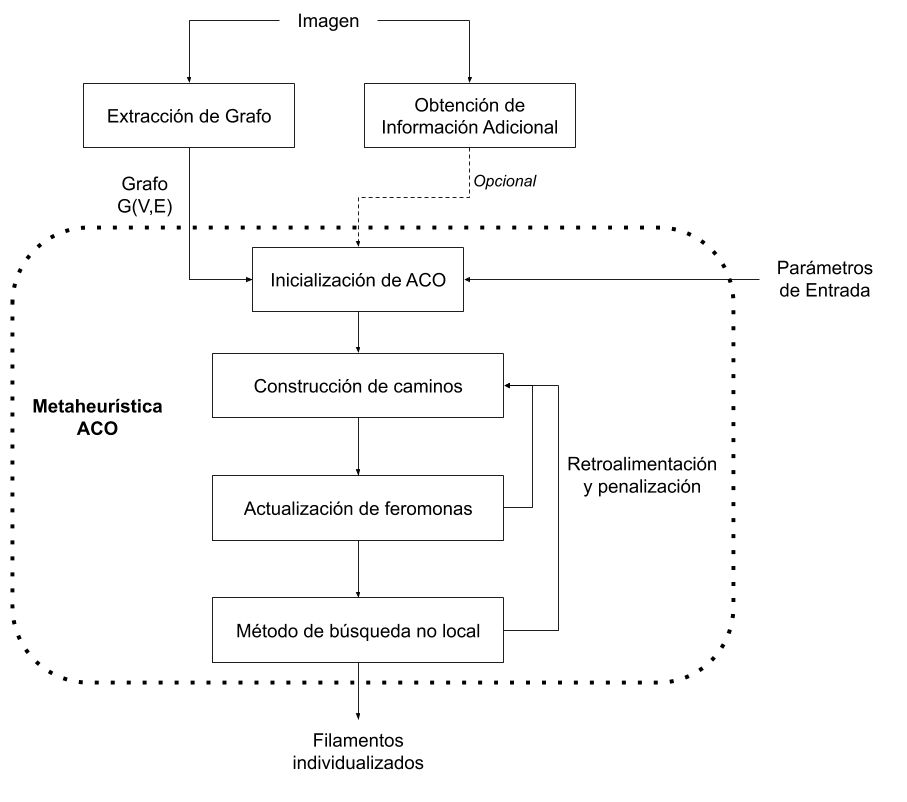
\includegraphics[scale=0.45]{imagenes/ACOdiagram.png}
    \caption[Diagrama de las etapas del algoritmo propuesto]{Diagrama simplificado de las etapas del algoritmo propuesto. Fuente: Elaboraci\'on Propia.}
    \label{fig:ACOdiagram}
\end{figure}

\section{Inicializaci\'on de la metaheur\'istica ACO}
\label{sec:acoInit}
En el paso de inicializaci\'on de ACO se deben definir los valores de los par\'ametros relacionados a las heur\'isticas y de las feromonas utilizadas. Una de las caracter\'isticas m\'as relevantes para discriminar aristas en el proceso de construcci\'on corresponde al \'angulo que forman 2 aristas adyacentes.
El primer umbral que permite definir si ambas aristas pertenecen al mismo filamento se define como $\theta$. As\'i, si el \'angulo se encuentra en el rango $[0, \theta]$ se puede dirimir que ambas aristas pertenecen al mismo filamento. Un segundo umbral se define como $Max\_Angle$, que indica el l\'imite por sobre el cual se puede inferir que estas 2 aristas no pertenecen al mismo filamento. Estos par\'ametros dependen de la c\'elula observada, asignando a $\theta$ valores de 30\textdegree ~para microt\'ubulos de planta y de 45\textdegree~ para neuronas. $Max\_Angle$ depende de $\theta$ al definirse como el m\'aximo entre 2.5 veces $\theta$ y 90\textdegree. El factor 2.5 es un valor obtenido experimentalmente que no ha sido sometido a sintonizaci\'on.

Otros par\'ametros a utilizar corresponden a {\it Max\_Axial\_Displacement} y a {\it Max\_Score}. El primero hace referencia a un par\'ametro de tolerancia que influye en 2 aspectos: al evaluar la curvatura general de una soluci\'on, y al evaluar la bifurcaci\'on entre 2 grupos de aristas al interior de la soluci\'on. La diferencia de la evaluaci\'on de bifurcaci\'on con respecto a la medici\'on de \'angulos entre aristas radica en que este criterio tambi\'en considera la magnitud de estos grupos de aristas. Los valores de {\it Max\_Axial\_Displacement} son de 1.5 para el caso de los microt\'ublos de planta o de 2.5 para las neuronas. Por su parte, {\it Max\_Score} define el puntaje m\'aximo a obtener por un camino de buena calidad. Su valor durante este trabajo corresponde a 2, y es utilizado por la heur\'istica miope (ecuaci\'on \ref{eq:heuristicaMiope}), que se define m\'as adelante en la secci\'on \ref{subsubsec:antTourInit}. A su vez, los par\'ametros $\alpha$ y $\beta$ tambi\'en utilizados en la heur\'istica miope, que regulan la ponderaci\'on entre esta heur\'istica y las feromonas, son fijados en 1.


En el caso de las feromonas, se define un valor inicial de $\tau_{ij} = 1$, pero utilizando un concepto inverso de feromona con respecto al que se present\'o previamente. El cambio consiste en el uso de {\it anti-feromonas} o SAP ({\it Substractive Anti-Pheromone}), definido por \citet{montgomery2002anti}, que se explica en la secci\'on \ref{subsec:pheroUpdate} y consiste en disminuir el valor de la feromona asociada a su respectiva arista. El uso de SAP introduce el par\'ametro $\gamma$, el que se define en 0.5 en base a lo encontrado en la literatura.

%%%%%%%%%%%%%%%%%%%%%%%%%%%%%%%%%%%%%%%%
%Para las feromonas se configura el valor inicial de $\tau_{ij}$ en 1 para los pares $\langle c_{ij}$,$ seg_{n}\rangle \> \forall c_{ij} \in \> ]\theta, Max\_Angle]$, dado que al usar SAP esta probabilidad se ir\'a reduciendo de acuerdo a un factor $\gamma$ seg\'un lo explicado en la secci\'on \ref{subsec:pheroUpdate}. El valor de $\gamma$ se define en 0.5, en base a lo encontrado en la literatura.
%%%%%%%%%%%%%%%%%%%%%%%%%%%%%%%%%%%%%

En cuanto al criterio de finalizaci\'on, este consiste en generar nuevas hormigas artificiales hasta que todas las aristas sean parte de al menos una soluci\'on de buena calidad, o que el n\'umero de hormigas generadas sea superior a 4 veces la cantidad de aristas. En lo que sigue de este trabajo se utiliza el t\'ermino hormigas en referencia a las hormigas artificiales o agentes.


El grafo que representa la red de caminos que pueden recorrer las hormigas se puede obtener mediante las herramientas descritas en la secci\'on \ref{subsec:infoLossSkel}, siendo {\it sknw} la seleccionada en esta investigaci\'on. Esta herramienta recibe como dato de entrada la imagen de microscop\'ia binarizada, realizando internamente el proceso de esqueletonizaci\'on y posterior transformaci\'on a una estructura de grafo.


\section{M\'etodo de construcci\'on de soluci\'on de cada hormiga}
\label{subsubsec:antTourInit}
Al comenzar un recorrido, cada hormiga es asignada una arista de acuerdo a la heur\'istica de asignaci\'on inicial, la que corresponde al primer elemento del camino o recorrido parcial $s^{P}$. La heur\'istica de asignaci\'on inicial analiza hasta 3 situaciones, dependiendo del tipo de c\'elula:
\begin{enumerate}
\item La arista a asignar debe tener al menos uno de sus nodos con grado 1, indicando que es el inicio o final de una parte del grafo.

\item De no haber aristas disponibles con esas caracter\'isticas, se realiza una asignaci\'on inicial de una arista que cumpla con 2 criterios:
\begin{itemize}
    \item Tener uno de sus nodos con grado 2 o superior.
    \item El \'angulo que forma la arista candidata a elegir, junto a otra arista a la que pertenece el nodo, debe pertenecer al rango $]\theta, Max\_Angle]$.
\end{itemize}
%$\theta$ es un umbral que define el \'angulo m\'aximo, en grados, bajo el que se considera que 2 aristas contiguas respetan la rectitud necesaria para formar parte del mismo filamento. $Max\_Angle$ es un umbral que define el \'angulo m\'aximo, en grados, por sobre el cual se descarta de forma absoluta que 2 aristas contiguas forman parte del mismo filamentos. Este rango delimita los pares de aristas que a priori no representan combinaciones que respetan el criterio de rectitud, pero cuya explicaci\'on puede encontrarse en variaciones inducidas durante la extracci\'on del grafo desde la imagen, por lo que es necesario incorporar la exploraci\'on de estos pares de aristas.

\item De no existir aristas con alg\'un nodo que cumpla con los dos criterios previos, es posible asignar una arista aleatoria. Esta arista no debe pertenecer al una soluci\'on o camino evaluado como de buena calidad. La calidad de un camino se presenta m\'as adelante en esta secci\'on.
\end{enumerate}

%a elecci\'on de un componente $c_{ij}$ por una hormiga durante la construcci\'on de un camino, se lleva a cabo mediante el c\'alculo de una probabilidad para cada componente $c_{ij}$ posible de elegir. Este conjunto de vecinos factibles se denomina $N(s^{P}) \subseteq C$. En la probabilidad de selecci\'on influye el camino ya escogido, denominado soluci\'on parcial $s^{P}$. 

% a diferencia de otros ACO, aca s^P != \emptyset al comienzo
Una vez asignada la primera arista seg\'un la heur\'istica previamente descrita, cada hormiga debe avanzar mediante la elecci\'on de nuevas aristas para a\~nadirlas a su recorrido. Este procedimiento corresponde a la probabilidad de elegir una arista o componente $c_{ij}$ a partir de un conjunto de aristas vecinas $N(s^{P})$. Las aristas que pertenecen a $N(s^{P})$ son solo las aristas adyacentes a la \'ultima arista agregada a la soluci\'on parcial $s^P$ que son factibles de agregar a la soluci\'on parcial. La factibilidad de a\~nadir una arista de $N(s^{P})$ a $s^{P}$ corresponde a la probabilidad expresada en la ecuaci\'on \ref{eq:antProbabilities}. Esta probabilidad depende del valor de la feromona $\tau_{ij}$ asociada a la arista $c_{ij}$, as\'i como del valor de la heur\'istica miope $\eta_{ij}$ (ecuaci\'on \ref{eq:heuristicaMiope}) que eval\'ua el \'angulo formando entre la arista $c_{ij} \in N(s^{P})$ y la \'ultima arista agregada a $s^{P}$, que se define como $s_{n}^{P}$.


En particular, la heur\'istica miope $\eta_{ij}$ entrega una puntuaci\'on que disminuye a medida que el \'angulo mencionado aumenta, siendo el rango $[0, \theta]$ el que otorga la puntuaci\'on m\'axima de $Max\_Score$. Si el \'angulo es mayor a $Max\_Angle$ la puntuaci\'on corresponde a 0. Para el rango intermedio $]\theta, Max\_Angle]$, la puntuaci\'on depende de la diferencia entre el \'angulo formando entre la arista $c_{ij} \in N(s^{P})$ y $s_{n}^{P}$. Mientras m\'as aumenta esta diferencia, menor es la puntuaci\'on asignada.


%que tiene asociada. Otro aspecto que influye en la elecci\'on de una arista es la desviaci\'on que puede ocasionar si se a\~nade a $s^P$, con respecto a la rectitud del camino ya recorrido. Esta evaluaci\'on se refleja en el valor $\eta_{ij}$ asociado a la arista, que se calcula mediante la heur\'istica miope. 
%mediante la heur\'istica miope (ecuaci\'on \ref{eq:heuristicaMiope}) que privilegia los candidatos que causen la menor desviaci\'on en la rectitud del camino. 
%Se define que las aristas $c_{ij}$ que aportan con mayor probabilidad a la menor desviaci\'on son aquellos que en conjunto con el \'ultimo elemento elegido por la hormiga en ese punto ($c_{(i-1)j}$) forman un \'angulo en el rango $[0, \theta]$. El criterio de finalizaci\'on para la hormiga corresponde a que el conjunto $N(s^{P}) = \emptyset$, es decir, que no existan opciones de aristas para seleccionar.

%P(C_{ij} | s^{P}) = P_{n_{i},n_{j}} = P_{e_{x}}
\begin{equation}
P(c_{ij} | s^{P}) = \frac
        {\tau_{ij}^{\alpha} ~ \eta_{ij}^{\beta}}
        {\sum\limits_{c_{ij}\in N(s^p)}{\tau_{ij}^{\alpha} ~ \eta_{ij}^{\beta} } }, \forall c_{ij} \in N(s^{P}).
\label{eq:antProbabilities}
\end{equation}

La evaluaci\'on de \'angulos entre aristas adyacentes que pertenezcan al rango intermedio $]\theta, Max\_Angle]$ en la heur\'istica miope, facilita la exploraci\'on de soluciones o caminos que de forma miope no califican como soluciones candidatas factibles de representar un filamento, pero que tampoco pueden ser descartados completamente. En el caso que un camino tenga uno o m\'as pares de aristas adyacentes cuyo \'angulo pertenezca a este rango, se definir\'a el camino como de {\it calidad intermedia}.

%Otro aspecto de la ecuaci\'on \ref{eq:heuristicaMiope} radica en la posibilidad de elecci\'on de aristas $c_{ij}$ que tienen un \'angulo en el rango $]\theta, \text{Max\_Angle}]$ con el componente de soluci\'on $c_{(i-1)j}$. Esto facilita la exploraci\'on de soluciones/caminos que de forma miope aparecen como de calidad no \'optima, y que para los efectos de este trabajo se denominan como de {\it calidad intermedia}. Esta evaluaci\'on consistente en disminuir la probabilidad de elecci\'on a medida que se incrementa la diferencia entre el \'angulo que forman $c_{ij}$ y $c_{(i-1)j}$, y la mitad de $\theta$.
%donde cada uno representa a una arista en esta investigaci\'on, y . Al momento de que la diferencia sea 90\textdegree, la probabilidad de asignaci\'on se reduce al 50\% de la probabilidad de un componente $c_{ij} \in [0, \theta]$.

\begin{equation}
    \eta_{ij} = 
        \begin{cases} 
        \text{Max\_Score si } \measuredangle(c_{ij}, s_{n}^{P}) \in [0, \theta],\\[3ex]
        
        \text{Max\_Score} \cdot \left(1 - \dfrac{ \left| \measuredangle(c_{ij}, s_{n}^{P}) - \frac{\theta}{2} \right|} {180} \right)  \text{ si } \measuredangle(c_{ij}, s_{n}^{P}) \in \quad ]\theta, \text{Max\_Angle}],\\[3ex]
        
        \text{0 en otro caso.}
        \end{cases}
    \label{eq:heuristicaMiope}
\end{equation}

Con la finalidad de cuantificar la calidad de la soluci\'on construida por una hormiga, en cada selecci\'on de arista realizada, se suma el resultado de la heur\'istica miope $\eta_{ij}$ a la calidad del camino que la hormiga lleva hasta ese punto. Cada hormiga comienza con una calidad 0, que al finalizar su recorrido es dividida por el n\'umero de aristas menos 1, para normalizar el valor entre las distintas soluciones. Se establece que para ser consideradas como una soluci\'on de {\it buena calidad}, la hormiga debe tener una calidad mayor o igual a $Max\_Score/2$. Es importante destacar que la calidad de una soluci\'on puede variar en cada etapa de la metaheur\'istica ACO, pudiendo descartarse una soluci\'on en base a los criterios de cada m\'etodo. El desechar una soluci\'on implica ajustar su calidad a 0, lo que la clasifica como de {\it mala calidad}. Las hormigas que en cada elecci\'on de arista hayan elegido componentes $c_{ij}$ que formaban un \'angulo en en rango $[0, \theta]$ con $s_{n}^{P}$, son las que obtienen el m\'aximo puntaje de $Max\_Score$ al normalizarse, y se definen como de {\it calidad \'optima}. Los caminos clasificados como de {\it calidad intermedia} son inicialmente parte del grupo de soluciones de buena calidad.

%Un planteamiento similar a lo anterior es el {\it Path Cover Problem} o PCP, en el que se descompone un grafo dirigido en caminos con el objetivo de obtener un conjunto de caminos. Cada nodo o arista debe pertenecer exactamente a un camino y los caminos pueden comenzar o terminar en cualquier parte del grafo.

%Esta reducci\'on del espacio de b\'usqueda debe considerar no eliminar soluciones o caminos v\'alidos, como puede suceder con casos de cruce o solapamiento de filamentos, o la existencia de ciclos. 


%En el caso de la individualizaci\'on de filamentos, es necesario que la definici\'on del problema considere como v\'alidos caminos que representen los casos de filamentos con o sin ciclos, as\'i como superposici\'on y/o cruce. Lo anterior impide forzar la pertenencia de un nodo o arista a un solo camino


\section{M\'etodo de actualizaci\'on de feromonas}
\label{subsec:pheroUpdate}
Una vez que la hormiga termina un recorrido, se eval\'ua su calidad para actualizar las feromonas $\tau_{ij}$ asociadas a los componentes de soluci\'on que lo conforman. As\'i, en una metaheur\'istica ACO tradicional, se aumenta el valor de $\tau_{ij}$ en cada $c_{ij}$ que es parte de un camino de buena calidad. Adicionalmente, los valores de las feromonas sufren decaimiento en el tiempo, dado por el par\'ametro $\rho$, que busca evitar la convergencia que las feromonas pueden causar en caminos de buena calidad obtenidos al inicio de las iteraciones.


En la individualizaci\'on de filamentos, se utilizan {\it anti-feromonas}, con el prop\'osito de indicar a las hormigas de futuras iteraciones los caminos que no son de buena calidad. La diferencia radica en que las anti-feromonas buscan acotar el espacio de soluciones $S$ sin necesariamente buscar la convergencia sobre un \'unico camino. Este cambio implica no utilizar el par\'ametro $\rho$, ya que no existe decaimiento en este uso de anti-feromonas, y reemplazarlo por el par\'ametro $\gamma$ como factor de reducci\'on/penalizaci\'on \citepxl{montgomery2002anti}. Al ser la penalizaci\'on un factor que se aplica sobre el valor de $\tau_{ij}$, la anti-feromona puede disminuir constantemente sin llegar a valer exactamente cero, por lo que se define un l\'imite de 2 penalizaciones como m\'aximo para cada anti-feromona. Al alcanzar este l\'imite, se reduce el valor de $\tau_{ij}$ a 0, haciendo imposible la elecci\'on de la arista $c_{ij}$ respectiva.
%para las hormigas cuya soluci\'on parcial $s^{P}$ contenga el segmento en el par $<$componente,segmento$>$ penalizado. 

Adem\'as de cambiar el uso de feromonas por el de anti-feromonas, se introduce una segunda modificaci\'on, relativa a las aristas a las que aplica la penalizaci\'on de las anti-feromonas. Un uso tradicional de anti-feromonas implica la disminuci\'on del valor de $\tau_{ij}$ para su respectiva arista $c_{ij}$, en caso de que se trate de un camino de mala calidad. 
Esto puede llevar a la p\'erdida de exploraci\'on de soluciones en la individualzaci\'on de filamentos, ya que una arista con un $\tau_{ij}$ penalizado por pertenecer a uno o m\'as caminos de mala calidad, puede bloquear otros caminos, dado que el valor de $\tau_{ij}$ no guarda relaci\'on con el conjunto de aristas que causa la penalizaci\'on. As\'i, las soluciones que pudiesen pasar por esa arista se ven limitadas.

 
%En aquel caso, la \'unica arista de $seg_{n+1}$ se transforma en un cuello de botella para la exploraci\'on debido a que penaliza de forma indiscriminada a todas las hormigas que pasen por ah\'i, independientemente del \'angulo que forme con otras aristas o componentes. Para subsanar aquel caso, a este tipo de segmentos se le a\~naden los nodos del segmento que lo precede, $seg_{n}$, con el objetivo de evitar que el an\'alisis del par $seg_{n+1}$ con la componente $c_{ij}$ que inicia el segmento $n+2$ sea solo de 2 aristas.

En este trabajo se propone que la penalizaci\'on de $\tau_{ij}$ guarde relaci\'on con el conjunto de aristas en el camino $s$ que preceden a la arista $c_{ij}$. Se define a aquel conjunto de aristas como un segmento de un camino recorrido por la hormiga $a$, expresado como $seg_{n}^{a}$. Los segmentos se generan durante la construcci\'on de un recorrido, existiendo siempre al menos un segmento en cada camino. Dado que el \'angulo entre 2 aristas adyacentes es uno de los criterios utilizados durante la construcci\'on de un camino, el fin de un segmento puede suceder en 2 casos: si la \'ultima arista en el camino corresponde al final del recorrido, o si la arista $s_{n}^{P}$ (la \'ultima arista agregada a $s^P$) forma un \'angulo en el rango $]\theta, Max\_Angle]$ con la arista $c_{ij} \in N(s^P)$ a agregar a la soluci\'on parcial.

\begin{figure}[h!]
    \centering
    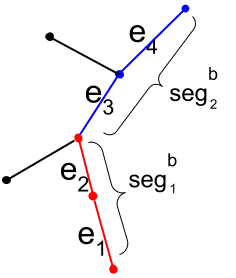
\includegraphics[scale=0.8]{imagenes/ant_segments_simple_case.png}
    \caption[Camino de una hormiga $b$ compuesto por 2 segmentos.]{Camino de una hormiga $b$ compuesto por 2 segmentos. El \'angulo entre las aristas $e_2$ y $e_3$ pertenece al rango $]\theta, Max\_Angle]$, finalizando el segmento $seg^{b}_1$ e iniciando el segmento $seg^{b}_2$. Fuente: Elaboraci\'on Propia.}
    \label{fig:segmentSimpleCase}
\end{figure}

As\'i, cada segmento esta formado por una o m\'as aristas, donde cada arista del segmento forma un \'angulo en el rango $[0, \theta]$ con sus vecinos. Un ejemplo de esto se puede observar en la Figura \ref{fig:segmentSimpleCase}, en el que si se penaliza la arista $e_3$, esta penalizaci\'on ser\'a asociada al segmento $seg^{b}_{1}$, disminuyendo la posibilidad de que futuras hormigas que recorran este segmento escojan $e_3$, sin perjuicio de otros caminos que pasen por $e_3$ pero no por el segmento $seg^{b}_{1}$.


Una ventaja de utilizar segmentos de camino es evitar volver a evaluar la relaci\'on entre todas las aristas que conforman el camino, ya que las aristas que conforman un segmento cumplen con un criterio para ser consideradas como parte del mismo filamento. As\'i, la evaluaci\'on de la calidad del camino se realiza solo en el caso que 2 aristas vecinas formen un \'angulo de rango intermedio ($]\theta, Max\_Angle]$), enfoc\'andose en las soluciones de calidad intermedia que permiten explorar el espacio de soluciones.


Se debe se\~nalar que esta propuesta de penalizaci\'on realiza la evaluaci\'on de la calidad del camino en orden inverso al utilizado durante la construcci\'on del recorrido, imitando el retorno que realiza una hormiga desde el alimento hacia su hormiguero. Esto, sumando al uso de segmentos, permite comenzar la revisi\'on en el \'ultimo par de aristas cuyo \'angulo pertenece al rango intermedio, es decir, el nodo donde termina el pen\'ultimo segmento y comienza el \'ultimo. A modo de ejemplo, en la Figura \ref{fig:segmentSimpleCase}, esto ser\'ia el nodo com\'un de las aristas $e_2$ y $e_3$, que separa los segmentos $seg^{b}_1$ y $seg^{b}_2$. En este ejemplo, en caso de penalizar la arista $e_3$, ser\'a solo disminuyendo su posibilidad de ser elegida para caminos que contengan al segmento $seg^{b}_1$ en su soluci\'on.

%cortar de atras para adelante una sola vez permite acotar los caminos malos sin descartar una solucion completamente, solo sacando la parte potencialmente mala al final


Por \'ultimo en este aspecto, y a diferencia del uso tradicional de feromonas o anti-feromonas, donde se penalizan todas las aristas pertenecientes a una soluci\'on, el recorrido inverso y el uso de segmentos permite que sea suficiente la penalizaci\'on de una arista en la soluci\'on para clasificar la soluci\'on $s$ como de mala calidad y desecharla. Esto permite que a partir de una soluci\'on de mala calidad se remueva el \'ultimo segmento, permitiendo a otra hormiga recorrer un camino similar con un distinto final, favoreciendo la exploraci\'on. Para visualizar esto, es posible utilizar la Figura \ref{fig:segmentComplexCaseH}, en donde una hormiga pudiese construir un camino incorporando las aristas $e_1$, $e_2$, $e_4$, $e_5$ y $e_6$. Al desechar el \'ultimo segmento, conformado solo por la arista $e_6$, permite que otra hormiga recorra desde $e_1$ hasta $e_5$, pudiendo agregar $e_7$ a su camino o terminando en $e_5$. 

\begin{figure}[h!]
    \centering
    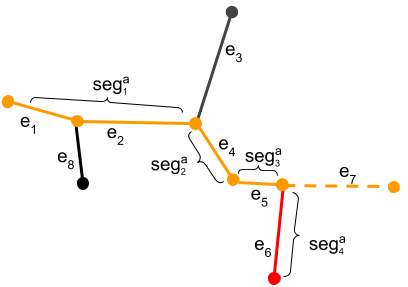
\includegraphics[scale=0.8]{imagenes/ant_segments_complex_case_H.png}
    \caption[Camino de una hormiga $a$ compuesto por 4 segmentos.]{Camino de una hormiga $a$ compuesto por 4 segmentos. El comienzo en orden inverso a la construcci\'on favorece la exploraci\'on, reemplazando el \'ultimo segmento por otro o simplemente concluyendo el recorrido. Fuente: Elaboraci\'on Propia.}
    \label{fig:segmentComplexCaseH}
\end{figure}

%Existen $N + 1$ segmentos en $s$ si la soluci\'on contiene $N$ elementos $c_{ij} \in ]\theta, 90]$ (de calidad intermedia). 
Lo anterior permite definir que la penalizaci\'on de $\tau_{ij}$ este asociada a la arista $c_{ij}$ y al segmento que precede a $c_{ij}$ en el recorrido de una hormiga $a$. El segmento que precede a $c_{ij}$ en un camino $s$ se define como $seg^{a}_{prev}$. Adicionalmente, se tiene que entre distintos caminos pueden existir segmentos equivalentes, lo que sucede en el caso de que contengan las mismas aristas. Esto permite que se refieran al mismo valor $\tau_{ij}$ a pesar de los nombres relativos al camino al que pertenecen. El funcionamiento del m\'etodo de penalizaci\'on propuesto se visualiza en la Figura \ref{fig:segmentComplexCase}.
 \begin{figure*}[t!]
    \centering
    \begin{subfigure}[t]{0.48\textwidth}
        \centering
        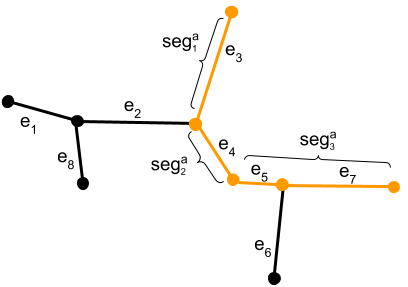
\includegraphics[height=2in]{imagenes/ant_segments_complex_case_1.png}
        \caption{Camino de una hormiga $a$ que contiene las aristas $e_3$, $e_4$, $e_5$ y $e_7$.}
        \label{fig:segmentComplexCase1}
    \end{subfigure}%
    ~ \hspace{0.5cm}
    \begin{subfigure}[t]{0.48\textwidth}
        \centering
        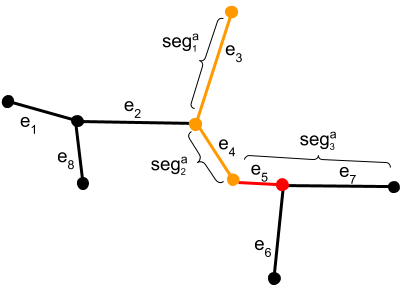
\includegraphics[height=2in]{imagenes/ant_segments_complex_case_2.png}
        \caption{Penalizaci\'on del camino de la hormiga $a$ en la arista $e_5$ con respecto al segmento $seg^{a}_2$ conformado solamente por la arista $e_4$.}
        \label{fig:segmentComplexCase2}
    \end{subfigure}

\vskip\baselineskip
    \begin{subfigure}[t]{0.48\textwidth}
        \centering
        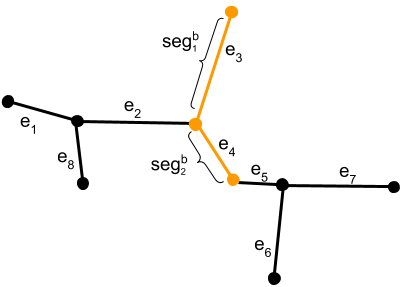
\includegraphics[height=2in]{imagenes/ant_segments_complex_case_4.png}
	    \caption{Camino de una hormiga $b$ que contiene las aristas $e_3$, $e_4$. El camino $b$ no puede agregar la arista $e_5$ debido a que se encuentra penalizada para el segmento formado por la arista $e_4$.}
        \label{fig:segmentComplexCase3}
    \end{subfigure}%
    ~ \hspace{0.5cm}
    \begin{subfigure}[t]{0.48\textwidth}
        \centering
        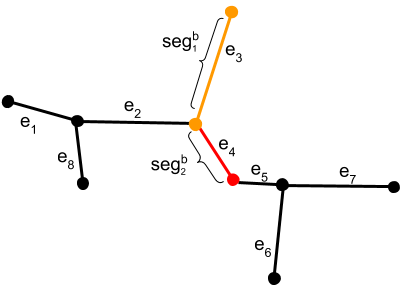
\includegraphics[height=2in]{imagenes/ant_segments_complex_case_5.png}
        \caption{Penalizaci\'on del camino de la hormiga $b$ en la arista $e_4$ con respecto al segmento $seg^{b}_1$ conformado solamente por la arista $e_3$.}
        \label{fig:segmentComplexCase4}
    \end{subfigure}

    \vskip\baselineskip

    \begin{subfigure}[t]{\textwidth}
        \centering
        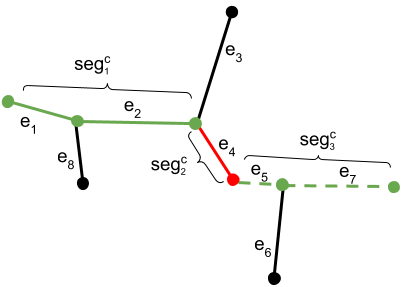
\includegraphics[height=2in]{imagenes/ant_segments_complex_case_block.png}
	    \caption{El camino de la hormiga $c$ no puede pasar de la arista $e_4$ en el caso que la penalizaci\'on no tenga relaci\'on con el segmento que precede a esa arista.}
        \label{fig:segmentComplexCaseBlocked}
    \end{subfigure}
    \caption[Funcionamiento de la propuesta de penalizaci\'on de anti-feromonas con segmentos y recorrido inverso.]{Funcionamiento de la propuesta de penalizaci\'on de anti-feromonas con segmentos y recorrido inverso. Por simplicidad se supone que la penalizaci\'on de $\tau_{ij}$ solo una vez es suficiente para eliminar la posibilidad de elegir una arista $c_{ij}$. En este ejemplo, los caminos $a$ y $b$ se desechan por evaluarse como de mala calidad. El camino es penalizando en $e_4$ respecto al segmento que lo precede. El camino $c$ puede seleccionar la arista $e_4$ ya que esta arista no se encuentra penalizada con respecto al segmento $seg^{c}_1$, pudiendo luego agregar el segmento $seg^{c}_3$. Fuente: Elaboraci\'on Propia.}
    \label{fig:segmentComplexCase}
\end{figure*}

Un caso particular en el que esta propuesta puede sufrir del mismo problema de bloqueo de soluciones, es al momento que un segmento formado por solo una arista se encuentre entre 2 segmentos. Este situaci\'on, reflejada en la Figura \ref{fig:segmentComplexCaseB}, implica que la penalizaci\'on que involucre un segmento de una sola arista, como el segmento $seg^{a}_2$, puede generar un bloqueo para los recorridos de otras hormigas. Este tipo de segmentos puede generarse a partir de aristas que forman un \'angulo que pertenece al rango $]\theta, Max\_Angle]$ con cada uno de sus vecinos, como es el caso de la arista $e_4$ en el ejemplo.

Para subsanar aquel caso, a los segmentos de solo una arista se le a\~naden las aristas del segmento que lo precede con el objetivo de evitar que el an\'alisis sea solo entre 2 aristas. As\'i, el segmento $seg^{a}_2$ pasa a ser formado por las aristas $e_3$ y $e_4$, evitando el bloqueo de la hormiga $b$.

\clearpage

%Este situaci\'on, reflejada en la Figura \ref{fig:segmentComplexCaseH}, implica que la penalizaci\'on efectuada a los caminos de las hormigas $a$ y $b$ pueden generar un bloqueo del camino de la hormiga $c$, dado que tras la penalizaci\'on efectuada en la evaluaci\'on de $b$, se tiene un segmento conformado solo por la arista $e_4$, la que forma un \'angulo que pertenece al rango $]\theta, Max\_Angle]$ con cada uno de sus vecinos.

%Si el camino continua siendo de .... otras hormigas pueden intentar iterativamente 
%explicar q la penalizacion es solo necesaria en soluciones de calidad intermedia


 \begin{figure*}[t]
    \centering
    \begin{subfigure}[t]{0.48\textwidth}
        \centering
        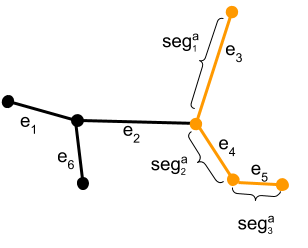
\includegraphics[height=2in]{imagenes/ant_segments_complex_case_B1.png}
        \caption{Camino de una hormiga $a$ que contiene las aristas $e_3$, $e_4$ y $e_5$.}
        \label{fig:segmentComplexCaseB1}
    \end{subfigure}%
    ~ \hspace{0.5cm}
    \begin{subfigure}[t]{0.48\textwidth}
        \centering
        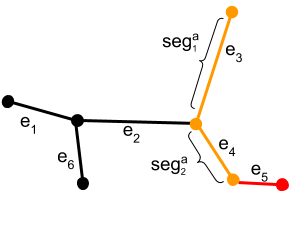
\includegraphics[height=2in]{imagenes/ant_segments_complex_case_B2.png}
        \caption{Penalizaci\'on del camino de la hormiga $a$ en la arista $e_5$ con respecto al segmento $seg^{a}_2$ conformado solamente por la arista $e_4$.}
        \label{fig:segmentComplexCaseB2}
    \end{subfigure}

\vskip\baselineskip
    \begin{subfigure}[t]{0.48\textwidth}
        \centering
        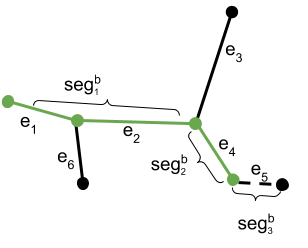
\includegraphics[height=2in]{imagenes/ant_segments_complex_case_B_blocked.png}
	    \caption{Camino de una hormiga $b$ que contiene las aristas $e_1$, $e_2,$ y $e_4$. El camino $b$ no puede agregar la arista $e_5$ debido a que se encuentra penalizada para el segmento conformado por la arista $e_4$, que corresponde al $seg^{a}_2$.}
        \label{fig:segmentComplexCaseBBlocked}
    \end{subfigure}%
    ~ \hspace{0.5cm}
    \begin{subfigure}[t]{0.48\textwidth}
        \centering
        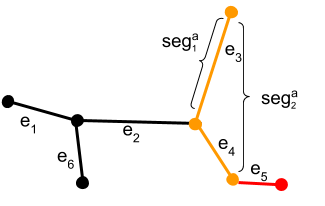
\includegraphics[height=2in]{imagenes/ant_segments_complex_case_B2_extended.png}
        \caption{Soluci\'on propuesta para los segmentos de solo 1 arista no causen bloqueos como el que afecta a la hormiga $b$, mediante la extensi\'on del segmento, a\~nadiendo el segmento anterior.}
        \label{fig:segmentComplexCaseB2Extended}
    \end{subfigure}

    \caption[Caminos de las hormigas $a$ y $b$.]{Caminos de las hormigas $a$ y $b$. Para evitar que la penalizaci\'on sobre $e_5$ por el segmento que lo precede, $seg^{a}_2$, bloquee el camino $b$, se modifica el inicio del segmento asociado a la penalizaci\'on, incorporando las aristas del segmento previo, $seg^{a}_2$. As\'i se mantiene la l\'ogica de asociar la penalizaci\'on no solo a la arista sino que tambi\'en al segmento que la precede. Estos casos suceden para aristas como $e_4$, que forman \'angulos en el rango $]\theta, Max\_Angle]$ con todas sus aristas vecinas, quedando solas en un segmento de largo 1. Fuente: Elaboraci\'on Propia.}
    \label{fig:segmentComplexCaseB}
\end{figure*}


%La perdida de exploraci\'on tambi\'en sucede en el caso que el segmento $seg_{n+1}$ contenga solo 1 arista y no sea el segmento en el que finaliza el recorrido de la hormiga. En aquel caso, la \'unica arista de $seg_{n+1}$ se transforma en un cuello de botella para la exploraci\'on debido a que penaliza de forma indiscriminada a todas las hormigas que pasen por ah\'i, independientemente del \'angulo que forme con otras aristas o componentes. 

%Luego, mediante la anti-feromona se relaciona un segmento $seg^{a}_n \subset s$ y la componente de soluci\'on $c_{ij} \in seg_{n+1} \in s$, donde la elecci\'on de la arista o componente $c_{ij}$ despu\'es de haber elegido las aristas pertenecientes a $seg_n$ origina una soluci\'on de mala calidad. 

\clearpage

\section{Criterios para la actualizaci\'on de anti-feromonas}

La anti-feromona se aplica sobre hormigas que han finalizado su recorrido, cuya calidad normalizada se encuentre entre $[Max\_Score/2, Max\_Score[$, las que tienden a ser caminos de calidad intermedia. Aquello implica que al menos un par de las aristas del recorrido forman un \'angulo que pertenece al rango intermedio $]\theta, Max\_Angle]$, necesitando un an\'alisis adicional para determinar si corresponde a una soluci\'on de buena calidad. Este an\'alisis consta de dos criterios que se aplican sobre todas las c\'elulas cuyos filamentos se deseen individualizar, mientras que existe un tercer criterio adicional aplicable solo en el caso de las neuronas. Los dos criterios generales, o criterios comunes, consisten en evaluar la curvatura del recorrido, como tambi\'en la magnitud del desplazamiento entre la proyecci\'on de un segmento con respecto a un segmento adyacente. El criterio adicional relativo solamente a las neuronas busca validar que la finalizaci\'on del recorrido no sea en una arista con uno de sus nodos con grado 1. Es decir, esta arista final no debe cumplir con el primer criterio de la heur\'istica de asignaci\'on de aristas iniciales, descrita en la secci\'on \ref{subsubsec:antTourInit}.
%El an\'alisis adicional se separa en evaluaciones comunes que no dependen de la c\'elula observada, agregando posteriormente las evaluaciones particulares.

\subsection{Curvatura de una soluci\'on}


La curvatura del recorrido de una hormiga $a$ se obtiene al calcular el \'angulo entre la proyecci\'on de un vector con respecto a otro. Los vectores son formados por el nodo inicial del camino, $v^{a}_1$, el centro de masa del recorrido de la misma hormiga, $mc^{a}$, y el nodo final, $v^{a}_n$. As\'i, se definen $\Vec{p} = v^{a}_1 - mc^{a}$ y $\Vec{q} = mc^{a} - v^{a}_n$.



%Estos vectores, definidos como $\Vec{p} = $ y $\Vec{q}$, se generan a partir d Corresponden a $\Vec{p}$ los elementos $v^{a}_1$ y $mc^{a}$, mientras que $\Vec{q}$ es formado por $mc^{a}$ y $v^{a}_n$.


El \'angulo entre la proyecci\'on de $\Vec{p}$ y $\Vec{q}$ no debe superar el valor que resulta al multiplicar el \'angulo $\theta$ por el factor {\it Max\_Axial\_Displacement}. Este factor permite flexibilizar la tolerancia de la curvatura en base a $\theta$. Si el recorrido de la hormiga tiene un \'angulo igual o mayor al umbral, implica que la soluci\'on encontrada es demasiado curva para representar un filamento, por lo que es penalizada y descartada. Un ejemplo se puede observar en la Figura \ref{fig:antCurvCase}, con el camino formado por las aristas $e_3$, $e_4$, $e_5$ y $e_7$, que presenta una curvatura muy marcada, por lo que es penalizado y descartado. La actualizaci\'on del valor de $\tau_{ij}$ mediante el criterio de curvatura se refleja en la ecuaci\'on \ref{eq:antiPheroSAP_Angle}.
%\begin{equation}
%    \label{eq:antiPheroSAP_Angle}
%    \tau_{ij} \leftarrow \tau_{ij} \cdot \gamma \quad \forall \langle c_{ij},seg_{n}\rangle > \textrm{Max\_Axial\_Displacement}
%\end{equation}

\begin{equation}
    \tau_{ij} \leftarrow
        \begin{cases}
        \tau_{ij} \cdot \gamma \text{ si } \measuredangle(proy(\Vec{p}), \Vec{q}) \geq \theta \cdot \text{Max\_Axial\_Displacement},\\[3ex]
        
        \text{0 si } \tau_{ij} \leq 0.25, \\[3ex]
        \tau_{ij} \quad \text{en otro caso.}
        \end{cases}
    \label{eq:antiPheroSAP_Angle}
\end{equation}

\begin{figure}[h]
    \centering
    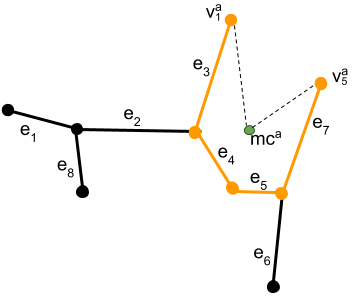
\includegraphics[scale=0.8]{imagenes/ant_curvature_case.png}
    \caption[Curvatura de un camino de una hormiga $a$ que contiene las aristas $e_1$, $e_3$, $e_4$ y $e_7$.]{Curvatura de un camino de una hormiga $a$ que contiene las aristas $e_1$, $e_3$, $e_4$ y $e_7$. $\Vec{p}$ es la proyecci\'on del vector formado por $v^{a}_1$ y $mc^{a}$. $\Vec{q}$ es el vector formado por $mc^{a}$ y $v^{a}_5$. Para cumplir con el rriterio de curvatura, el \'angulo entre la proyecci\'on de $\Vec{p}$ y $\Vec{q}$ debe ser menor a $\theta \times Max\_Axial\_Displacement$ para no descartar la soluci\'on. }
    \label{fig:antCurvCase}
\end{figure}

\begin{figure*}[h]
    \centering
    \begin{subfigure}[t]{0.45\textwidth}
        \centering
        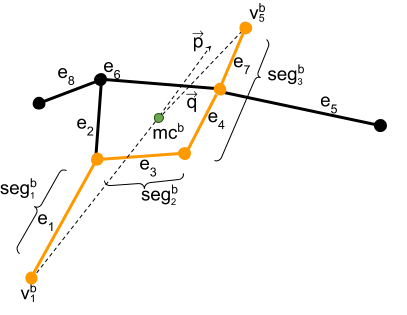
\includegraphics[height=2.5in]{imagenes/ant_segmentMagnitude_case.png}
        \caption{Soluci\'on $b$ cumple con el criterio de curvatura, pero la proporci\'on de la magnitud entre los segmentos $seg^{b}_2$ y $seg^{b}_1$ con respecto a su \'angulo puede indicar que no es una buena soluci\'on.}
        \label{fig:antCurvNotEnough}
    \end{subfigure}
    ~ \hspace{0.5cm}
    \begin{subfigure}[t]{0.45\textwidth}
        \centering
        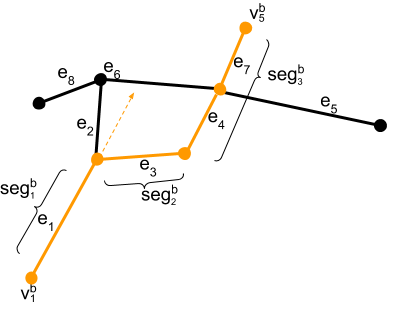
\includegraphics[height=2.5in]{imagenes/ant_segmentMagnitude_case_2.png}
        \caption{An\'alisis del desplazamiento del segmento $seg^{b}_2$ con respecto a la proyecci\'on del $seg^{b}_1$ denota un giro brusco y pronunciado que podr\'ia no respetar la rigidez de algunos tipos de filamentos.}
        \label{fig:antMaxDisplExample}
    \end{subfigure}%
    \caption[Criterio de magnitud y pronunciaci\'on del desplazamiento entre 2 segmentos contiguos.]{Criterio de magnitud y pronunciaci\'on del desplazamiento entre 2 segmentos contiguos. (a) El criterio de curvatura puede no ser suficiente por si mismo para descartar todas las soluciones de mala calidad. (b) La informaci\'on a priori respecto a la rigidez de un filamento permite descartar soluciones que presenten cambios demasiado pronunciados entre los segmentos que la conforman. Fuente: Elaboraci\'on Propia.}
    \label{fig:antMaxDisp}
\end{figure*}

\subsection{Magnitud de desplazamiento entre segmentos}
%agregar referencia? tindemans rod straightness \cite{hawkins2010model} of MTs o 
El an\'alisis respecto a la magnitud del desplazamiento entre la proyecci\'on de un segmento en relaci\'on a sus segmentos vecinos se fundamenta en la rigidez que algunos tipos de filamentos como los microt\'ubulos y los filamentos de actina poseen \citepxl[ver\hspace{0.1cm} ]{stam2017filament, civalek2011bending}. El criterio de m\'aximo desplazamiento entre segmentos contiguos consiste en limitar la magnitud del movimiento que representa un segmento en relaci\'on al \'angulo que forma con sus segmentos adyacentes. Esto permite descartar soluciones que respeten el criterio de curvatura, pero que presentan movimientos pronunciados que sobrepasan la rigidez esperada de un filamento.

%El criterio de rigidez consiste en analizar los segmentos con respecto a la totalidad de sus predecesores, comenzando por el \'ultimo segmento recorrido por la hormiga, es decir, desde el extremo final de la soluci\'on. 
A partir de cada par de segmentos vecinos en una soluci\'on, se  selecciona el segmento de mayor longitud, el que servir\'a para determinar cual es el movimiento proyectado con respecto al movimiento reflejado por el segmento de menor longitud. Se define el segmento m\'as largo entre ambos segmentos comparados en un camino $a$ como $seg^{a}_{iMax}$ , mientras que el segmento menor es $seg^{a}_{jMin}$. El \'angulo entre $seg^{a}_{jMin}$ y la proyecci\'on de $seg^{a}_{iMax}$ se define como 
$\measuredangle seg^{a}_{pMaxMin}$ por simplicidad. En el caso de que el \'angulo $\measuredangle seg^{a}_{pMaxMin}$ este en el rango $[0, \theta]$ se entiende que se respeta el criterio de m\'aximo desplazamiento.


Si el \'angulo es mayor a $\theta$, se espera que la magnitud del segmento menor $seg^{a}_{jMin}$ multiplicada por el seno de $\measuredangle seg^{a}_{pMaxMin}$ sea menor al umbral que delimita al desplazamiento m\'aximo entre segmentos, definido como el m\'ultiplo de $seg^{a}_{iMax}$ por el 10\% de {\it Max\_Axial\_Displacement}. Lo anterior se ilustra en la Figura \ref{fig:antMaxDisp}, y se describe la actualizaci\'on de $\tau_{ij}$ en la ecuaci\'on \ref{eq:antiPheroSAP_Axial}.

% como $s_{max} = \max(\norm{seg_{n}}, \norm{seg_{1,n-1}})$, para calcular el \'angulo suplementario que forma con respecto al otro miembro del par, definido como $s_{min}$. El \'angulo suplementario, $\measuredangle supl(s_{max},s_{min})$ es el equivalente a calcular el \'angulo entre la proyecci\'on de $s_{max}$ y $s_{min}$.

\begin{equation}
    \tau_{ij} \leftarrow
        \begin{cases}
        \begin{split}
         \tau_{ij} \cdot \gamma \text{ si } & \sin(\measuredangle seg^{a}_{pMaxMin}) > seg^{a}_{iMax} \cdot 0.1 \cdot \text{Max\_Axial\_Displacement} \\ & \land \measuredangle seg^{a}_{pMaxMin}) > \theta,
        \end{split}
        \\[3ex]
        
        \text{0 si } \tau_{ij} \leq 0.25, \\[3ex]
        \tau_{ij} \quad \text{en otro caso}.
        \end{cases}
    \label{eq:antiPheroSAP_Axial}
\end{equation}

%Luego $s_{min}$ es multiplicado por el seno del \'angulo suplementario, estableciendo el desplazamiento con respecto al eje que forma $s_{max}$ y su proyecci\'on. El umbral que delimita al desplazamiento calculado previamente se define como el m\'ultiplo de $s_{max}$ por 10\% de {\it Max\_Axial\_Displacement}. 

%Si el \'angulo suplementario es menor a $\theta$, se puede declarar que se cumple el criterio de rigidez. Lo anterior se refleja en la ecuaci\'on \ref{eq:antiPheroSAP_Axial}. 


%Esta propiedad puede ser utilizada para delimitar como un segmentos de una hormiga se relaciona con el resto de la soluci\'on, ya que estos ser\'ia un reflejo indirecto de los movimientos din\'amicos de un filamento en el tiempo, capturados en un punto a trav\'es de una imagen. 
%La rigidez de un filamento puede describirse mediante la relaci\'on que existe entre un segmento de una hormiga, con respecto a todos los segmentos que lo preceden. 


\subsection{Criterio espec\'ifico para neuronas}
\label{subsec:pheroNeurons}

%Si un camino cumple con ambas criterios de penalizaci\'on comunes, y se trata de una c\'elula distinta a una neurona, la soluci\'on avanza hac\'ia el an\'alisis del m\'etodo de b\'usqueda no local. En cambio,
Si la c\'elula observada es una neurona, corresponde aplicar el criterio adicional espec\'ifico a esta c\'elula. Este criterio adicional se fundamenta en que el comportamiento esperado de los filamentos en una neurona permite caracterizar los lugares desde los cuales nuevos filamentos pueden generarse. As\'i, es necesario validar que los filamentos de una neurona parten del {\tt soma} o centro de la misma, y que filamentos posteriores que no comiencen del soma solo pueden nacer a partir de otros filamentos. Un camino que termine en un nodo final de grado de 1 no respeta aquel comportamiento, debido a que en un grafo que representa una red de filamentos de una neurona, los nodos ubicados en el soma o en la intersecci\'on entre filamentos presentan un grado mayor a 1. La penalizaci\'on al valor de $\tau_{ij}$ para este caso particular se refleja en la ecuaci\'on \ref{eq:antiPheroSAP_neuron}.

\begin{equation}
    \tau_{ij} \leftarrow
        \begin{cases}
         \tau_{ij} \cdot \gamma \text{ si } deg(v^{a}_{n}) = 1,  \\[3ex]
        
        \text{0 si } \tau_{ij} \leq 0.25, \\[3ex]
        \tau_{ij} \quad \text{en otro caso}.
        \end{cases}
    \label{eq:antiPheroSAP_neuron}
\end{equation}

%Finalmente, la ecuaci\'on \ref{eq:antiPheroSAP} refleja la aplicaci\'on de las {\it anti-feromonas} sobre el par $\langle c_{ij}$,$ seg_{n}\rangle \forall c_{ij} \in ]\theta, Max\_Angle]$  donde $c_{ij} \in seg_{n+1}$, y cuya elecci\'on dio lugar a $seg_{n+1}$ que se aleja del desplazamiento axial m\'aximo que un filamento puede soportar.



\section{M\'etodo de b\'usqueda no local}
\label{sec:nonLocalSearch}
Una vez que la hormiga termina un recorrido, es posible agregar un m\'etodo de retroalimentaci\'on sobre la calidad del camino construido, basado en l\'ogicas globales/centralizadas que escapan de la b\'usqueda local que realiza cada hormiga. El o los m\'etodos en esta etapa permite extender la l\'ogica con respecto a una metaheur\'istica ACO, y son opcionales, por lo que no siempre son utilizados. 

Para la individualizaci\'on de filamentos, la evaluaci\'on global corresponde a eliminar soluciones candidatas que no aporten informaci\'on nueva, como puede suceder si una soluci\'on se encuentra contenida dentro de otra. Espec\'ificamente, si una soluci\'on $s^{a}$ se conforma por uno o m\'as segmentos y todos estos existen de forma equivalente en otra soluci\'on $s^{b}$, que a su vez puede tener segmentos que no posean equivalencia en $s^{a}$, se cumple que $s^{b}$ contiene a $s^{a}$. Al ser una soluci\'on contenida en otra, $s^{a}$ es redundante, pudiendo descartarse al disminuir su calidad a 0. En el caso que $s^{a}$ y $s^{b}$ sean id\'enticas, se conserva la soluci\'on que se haya construido primero. 
 
%\begin{itemize}
%    \item $\forall seg^{a}_{i} \in s^{a}, i = 1\dots n$
    
%    \item $s^{a} \subseteq s^{b}$
%\end{itemize}

Mediante la comparaci\'on de segmentos equivalentes, esta revisi\'on centralizada busca evitar recorridos con un bajo n\'umero de aristas, especialmente los caminos de 1 arista. Un potencial problema asociado a este m\'etodo se encuentra en el caso de que la solucion descartada, $s^{a}$ en el ejemplo, sea la que representa de mejor forma a un filamento, y que la soluci\'on restante por ende sea una representaci\'on no exacta.
%RIESGO ASOCIADO a overmatch!!

%Si dos soluciones, $s_i$ y $s_j$ de las hormigas $i$,$j$, conformadas solamente por componentes $c_{ij} \in [0, \theta]$  (todos los componentes son de {\it buena calidad}), y que adem\'as eran la \'unica opci\'on posible en cada avance de la hormiga (probabilidad 1 de ser elegidas)
%tal que $s_i \subseteq s_j$ o viceversa, se tiene que una soluci\'on candidata no aporta nueva informaci\'on.

\section{Extracci\'on de informaci\'on para individualizar filamentos}
Previo al uso de la metaheur\'istica ACO para individualizar filamentos, es necesario recabar la mayor cantidad de informaci\'on posible a partir de la imagen, as\'i como del grafo extra\'ido. Adem\'as se debe considerar la incorporaci\'on de informaci\'on espec\'ifica de los filamentos en la c\'elula observada, como el o los comportamientos esperados de estos, las que pueden conocerse previamente a la ejecuci\'on del algoritmo propuesto. A medida que se obtiene m\'as informaci\'on, es posible incorporar en el algoritmo diversas heur\'isticas que permitan acotar el espacio de b\'usqueda.

Como se observa en el cap\'itulo \ref{chap:stateoftheart}, diversas investigaciones obtienen informaci\'on geom\'etrica o topol\'ogica, por lo general a partir de una imagen de filamentos. Para extender la obtenci\'on de informaci\'on topol\'ogica con respecto a otros m\'etodos, es posible utilizar los algoritmos para grafos existentes en la librer\'ia {\it sknw}, que son las implementaciones de algoritmos conocidos para grafos. As\'i, es posible utilizar un algoritmo de centralidad como {\it closeness centrality}, el que calcula la distancia de cada nodo con respecto a lo dem\'as, permitiendo identificar los que se encuentran a la menor distancia de todos.


La relevancia de esta informaci\'on adicional es directa en el caso de las neuronas, siendo utilizada en la seccion \ref{subsec:pheroNeurons}, mientras que puede requerir de an\'alisis adicional por parte de expertos para otros filamentos. La aplicaci\'on del algoritmo {\it closeness centrality} refleja la posibilidad de expandir y/o incrementar el uso de informaci\'on topol\'ogica en el algoritmo propuesto. Un ejemplo de {\it closeness centrality} para filamentos en neuronas y microt\'ubulos se observa en la Figura \ref{fig:ExtraInfoCenterNodes}, en la que se eligieron los 3 nodos con menor distancia a los dem\'as. Luego, el color magenta refleja las aristas que poseen al menos uno de estos nodos, mientras que las aristas en amarillo indican las que no poseen ninguno.
%entrega informaci\'on relevante respecto a la conectividad interna en conjuntos de filamentos.

 \begin{figure*}[h!]
    \centering
    \begin{subfigure}[t]{0.48\textwidth}
        \centering
        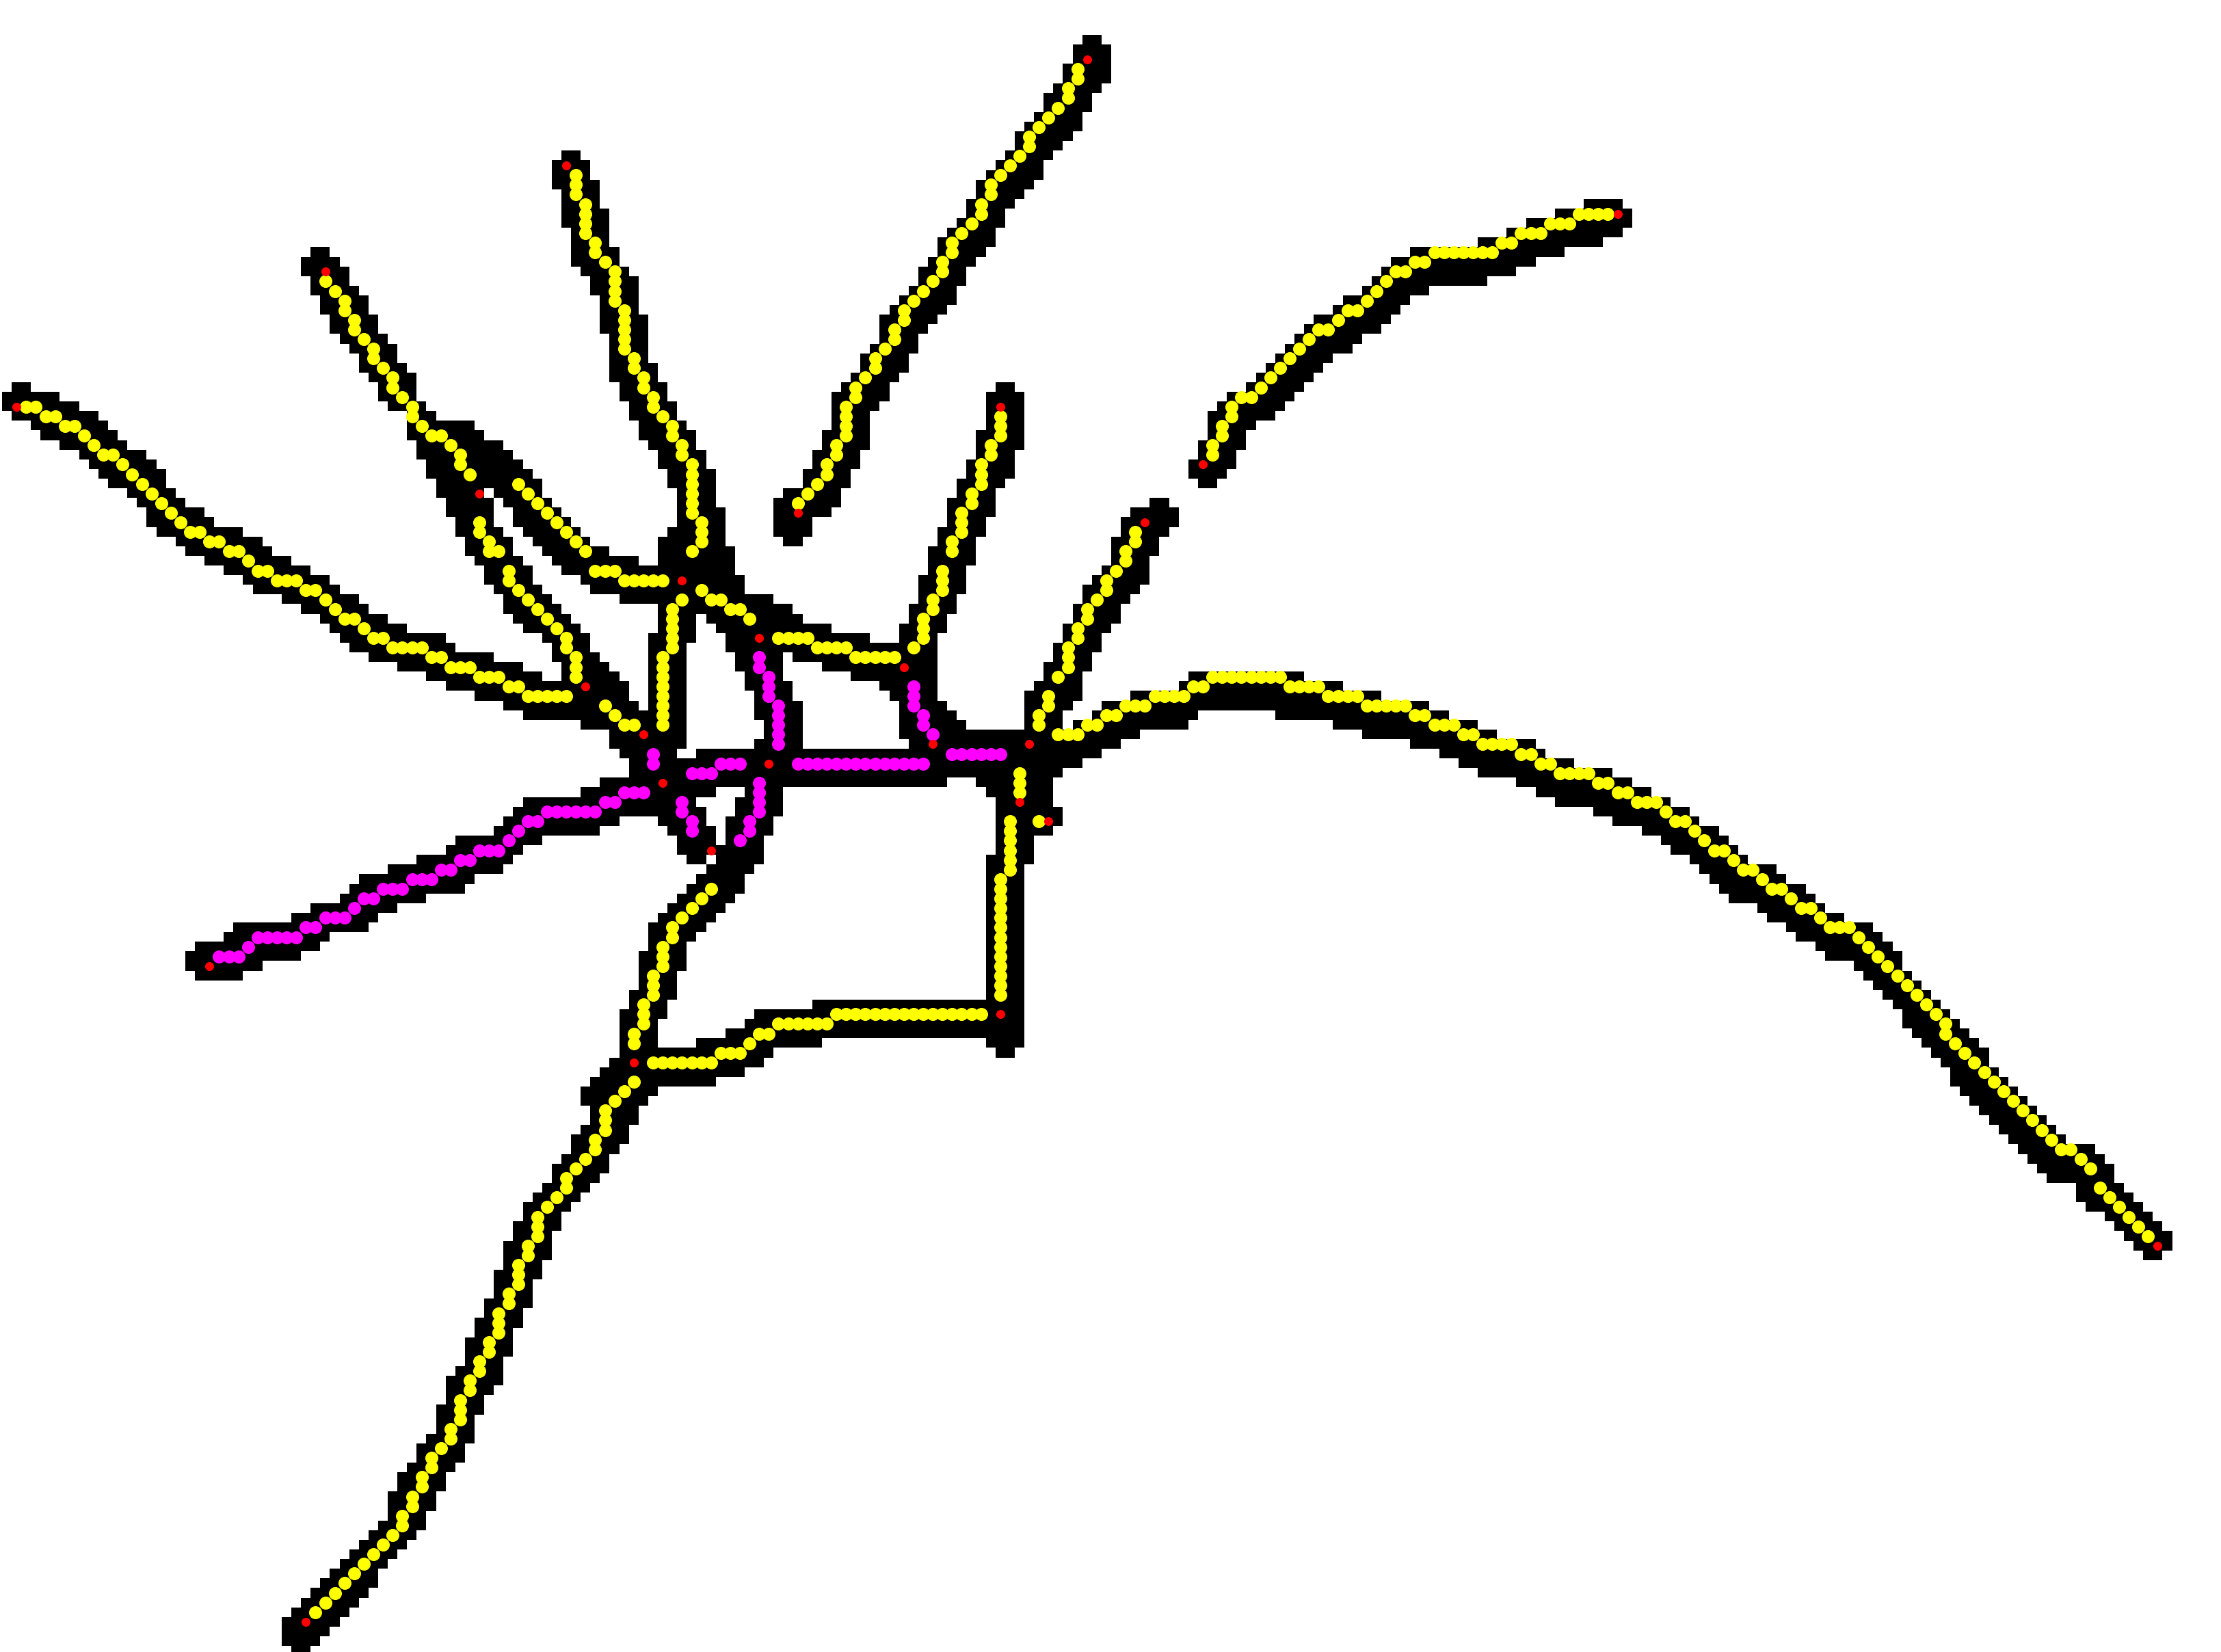
\includegraphics[height=2in]{imagenes/50-ROIs-Spinning-Marchantia-somaEdges.png}
        \caption{Uso del algoritmo {\it closeness centrality} en un grupo de microt\'ublos }
        \label{fig:SpinningCenterNodes}
    \end{subfigure}%
    ~ \hspace{0.5cm}
    \begin{subfigure}[t]{0.48\textwidth}
        \centering
        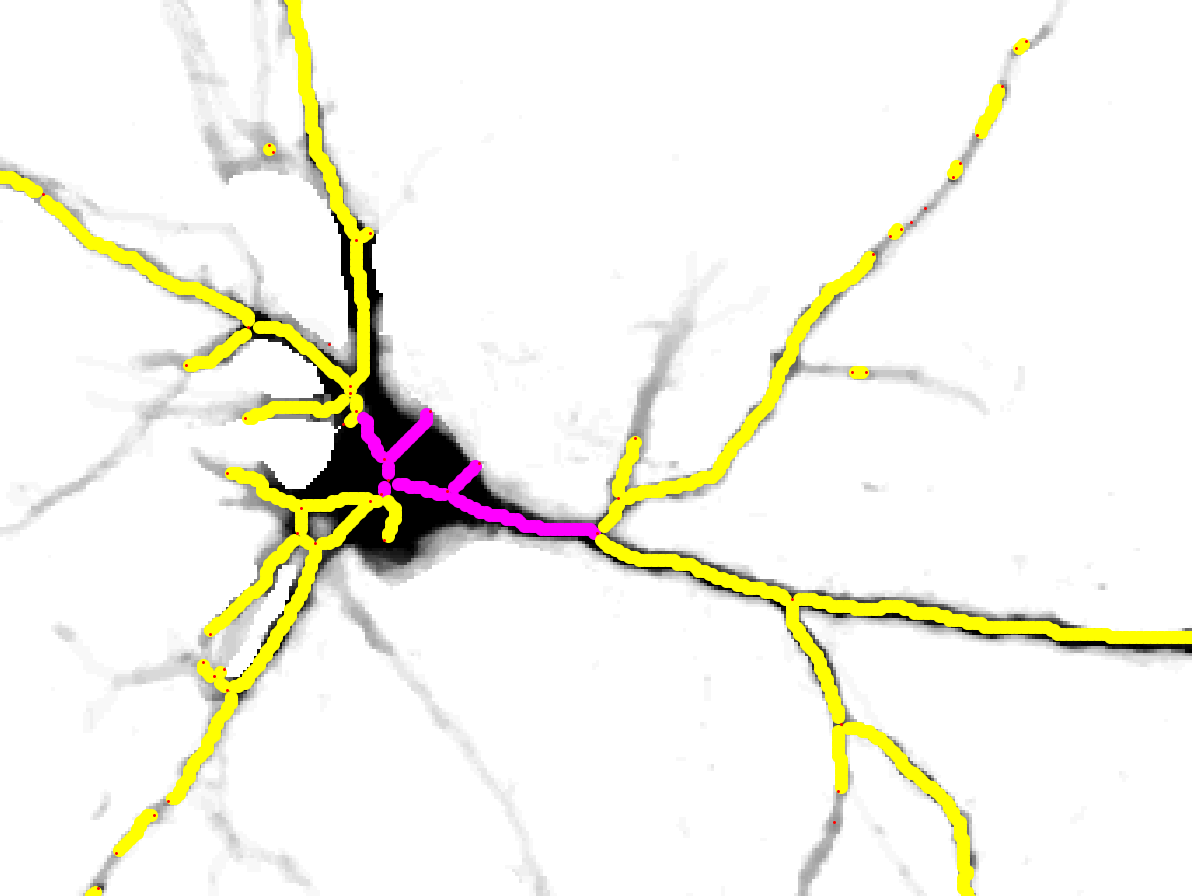
\includegraphics[height=2in]{imagenes/Porta18-3a1-somaEdges.png}
        \caption{Uso del algoritmo {\it closeness centrality} para reflejar nodos y aristas centrales, las que pueden corresponder a la secci\'on del soma en una neurona.}
        \label{fig:Porta18SomaNodes}
    \end{subfigure}

    \caption[Ejemplo del algoritmo {\it closeness centrality} eligiendo los 3 nodos con menor distancia a los dem\'as nodos.]{Ejemplo del algoritmo {\it closeness centrality} eligiendo los 3 nodos con menor distancia a los dem\'as nodos. El color magenta indica que aristas poseen al menos uno de estos 3 nodos. En el caso de una neurona, permite asociar una o m\'as aristas a una secci\'on espec\'ifica como el soma. Fuente: Elaboraci\'on Propia.}
    \label{fig:ExtraInfoCenterNodes}
\end{figure*}

%info espacial: Ejemplo within, analisis de cruces. Intersect, disjoin y otros, en postgis
Adem\'as de la extracci\'on de informaci\'on previo al uso de la metaheur\'istica ACO, es posible realizar de manera similar, la obtenci\'on de informaci\'on durante la individualzaci\'on de filamentos. Un ejemplo de esto es la informaci\'on espacial con respecto a los nodos y aristas que pueden ser elegidas como parte de un camino. La informaci\'on espacial facilita la comparaci\'on y el an\'alisis entre caminos para identificar casos de cruce, intersecci\'on o solapamiento. En particular, en la secci\'on \ref{sec:nonLocalSearch} se utiliza la consulta espacial {\it within} disponible en la extensi\'on espacial {\it Postgis} para la base de datos {\it PostgreSQL}, para comparar la informaci\'on distinta que entrega un camino con respecto a los dem\'as, considerando que puede existir repetici\'on de caminos entre distintas hormigas. Este an\'alisis resulta simple a trav\'es de una consulta espacial, especialmente a medida que aumentan los caminos a comparar.

El uso de informaci\'on geom\'etrica, topol\'ogica y espacial, repartidos en los m\'etodos de la metaheur\'istica ACO, se enfocan en ampliar las opciones de an\'alisis que puede realizar un experto, as\'i como aumentar la precisi\'on de la individualizaci\'on de filamentos. Nuevas caracter\'isticas que modifiquen la exploraci\'on del espacio de soluciones pueden ser a\~nadidas en el m\'etodo de construcci\'on de soluciones, ampliando el criterio que solamente utiliza el \'angulo para determinar o descartar con certeza que 2 aristas pertenezcan o no al mismo filamento. A su vez, en este mismo m\'etodo es posible incorporar nuevas condiciones que delimiten con mayor detalle el inicio o final de un camino.
Por su parte. agregar restricciones adicionales que penalicen caminos finalizados puede realizarse tanto en el m\'etodo de actualizaci\'on de feromonas, en caso de que se trate de restricciones que no requieran comparaci\'on con otras hormigas, o en el m\'etodo de b\'usqueda no local para comparaciones entre 2 o m\'as hormigas.

\section{Ponderaci\'on de Caracter\'isticas}
\label{subsec:ponderacion}
El algoritmo propuesto desarrollado para la individualizaci\'on de filamentos considera el uso de caracter\'isticas espaciales, topol\'ogicas y geom\'etricas, cuyo uso puede variar dependiendo de la c\'elula representada por el grafo extra\'ido, as\'i como la etapa de la metaheur\'sitca ACO en la cual se aplican. La etapa de construcci\'on de soluciones emplea el \'angulo entre aristas vecinas para definir la posibilidad de elecci\'on que cada hormiga tiene al ir avanzando. En esta etapa tambi\'en se aplica la heur\'istica de asignaci\'on inicial, en la que influye el grado de los nodos para determinar la arista inicial de cada camino. Por su parte, en el m\'etodo de actualizaci\'on de feromonas se usan las caracter\'isticas geom\'etricas como la curvatura del filamento y la diferencia en la magnitud entre segmentos contiguos, agreg\'andose el uso de informaci\'on topol\'ogica obtenida con el algoritmo de centralidad en grafos {\it closeness centrality}, en el caso de las neuronas. En cuanto al m\'etodo de b\'usqueda no local, se utiliza informaci\'on espacial para descartar soluciones que presenten informaci\'on repetida con respecto a otras soluciones.


Dado que las diversas caracter\'isticas utilizadas en el algoritmo propuesto se encuentran en distintos m\'etodos de la metaheur\'istica ACO, no es posible utilizar un \'unico par\'ametro para obtener una ponderaci\'on directa. En cambio, se propone un criterio para su ponderaci\'on basado en otorgar $\frac{1}{3}$ del peso a cada etapa del modelo, distribuyendo aquel valor internamente dependiendo de si la caracter\'istica se utiliza por s\'i sola o en combinaci\'on con otra, as\'i como considerando si el uso es repetitivo durante la ejecuci\'on de la etapa o solo se realiza una vez por etapa. Lo anterior permite establecer la siguiente ponderaci\'on:

\begin{itemize}
    \item Construcci\'on de soluciones: $\frac{100}{n}$\% el grado de los nodos, y el remanente para el \'angulo entre aristas, con $n$ como el n\'umero de aristas.
    \item M\'etodo de b\'usqueda no local: 100\% posici\'on de la arista.
    \item Actualizaci\'on de feromonas: 50\% curvatura, 50\% diferencia de magnitud entre segmentos. En el caso espec\'ifico de las neuronas, corresponde a $33.\overline{3}\%$ curvatura, $33.\overline{3}\%$ diferencia de magnitud entre segmentos y $33.\overline{3}\%$ informaci\'on topol\'ogica de centralidad.
\end{itemize}

Durante la construcci\'on de soluciones, el grado de los nodos solo se utiliza en la heur\'istica de asignaci\'on de la primera arista, por lo que para caminos de una sola arista corresponde a la totalidad de la ponderaci\'on de la etapa. A medida que crece el n\'umero de aristas, su peso va disminuyendo gradualmente al irse traspasando al criterio de \'angulo entre aristas. En cuanto a la diferencia de magnitud entre segmentos, esta se conforma en partes iguales del \'angulo entre segmentos y del uso de la magnitud de los mismos.

\vspace{1cm}
En resumen, las condiciones del problema de identificaci\'on de filamentos dan pie a establecer su representaci\'on mediante un problema de optimizaci\'on de restricciones (COP), estando el modelo para la resoluci\'on del COP basado en la metaheur\'istica ACO para su resoluci\'on. La implementaci\'on del algoritmo propuesto que resuelve el COP basado en la metaheur\'istica ACO se encuentra escrito en C++.